\section{Results}
\label{sec:results}



\subsection{Specific answers are sparse over memories}
\label{sec:scarcity}
\begin{figure}[t]
\centering
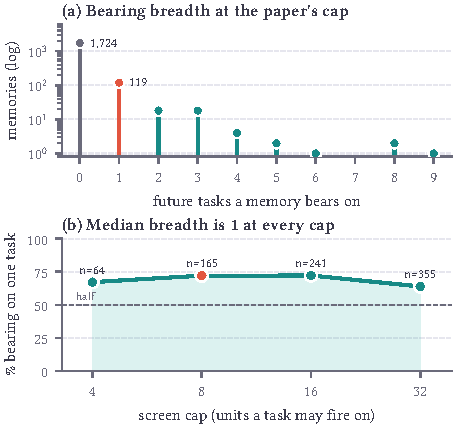
\includegraphics[width=\columnwidth]{fig_sparse}
\caption{Answer bearing is sparse at every screen cap (exploratory).
\textbf{(a)}~Number of memory units (of $\bearUnits$) that bear on each count of
screened future tasks, at the paper's cap of eight units per task (log axis).
\textbf{(b)}~Share of bearing memories that bear on exactly one task when the
cap is 4, 8, 16 or 32 units; $n$ is the number of bearing memories. The median
breadth is one at every cap.}
\label{fig:sparse}
\Description{Two panels. Top: a log-scale histogram of how many tasks each memory bears on, with 1,724 memories at zero and 119 at one, falling quickly after. Bottom: at screen caps of 4, 8, 16 and 32, between 64 and 72 percent of bearing memories bear on exactly one task.}
\end{figure}
Screening all 1{,}889 memory units against the 295 deterministically scored
questions yields 75 discriminative tasks: questions for which the screen fires
on at least one and at most eight units of the domain pool. Over those tasks,
165 memories bear on at least one, across 266 memory--task edges, and the
distribution is concentrated at one (Figure~\ref{fig:sparse}a): 119 memories
bear on exactly one task, 18 on two and 18 on three, with a tail reaching
nine. \emph{Among the 165 memory units that bear on at least one of the 75 qualifying
tasks, the median bears on one}; the other 1{,}724 units bear on none, so this
is not a median over all 1{,}889 units. Only 46 memories bear on two or more
tasks, and they come from 23 source trajectories, so they are not 46
independent draws; we report episode-clustered intervals wherever this
matters.

These are screen statistics, not re-execution results. The screen's cap of
eight units is what makes it specific: of the 220 deterministic questions it
excludes, $\soScrZero$ fire on no unit and $\soScrOver$ on more than eight,
often because short answers, such as a single number or letter, occur on many
pages. Without the cap, string containment alone fires for every one of
the $\soNoCapMems$ memories, on $\soNoCapMin$ to $\soNoCapMax$ tasks each. The pattern persists across the tested caps: at 4, 8, 16 and 32 units,
the median answer-bearing memory bears on exactly one task, and
$\rvCapShareLo$--$\rvCapShareHi\%$ bear on exactly one
(Figure~\ref{fig:sparse}b). The
sparsity we report therefore concerns \emph{specific} answers in this
benchmark, with these memory units and tasks. The screen does not identify
all useful pairs: cells outside \textsc{bearing} contribute more helped cells ($\raNonBearHelped$) than
bearing cells do (50), most at the perturbation floor
(Section~\ref{sec:metrics}), and the gold-free screen's picks lift accuracy from
$\gfWithoutPct\%$ to $\gfWithPct\%$ on cells the gold screen never selected
(Section~\ref{sec:screen}). A gold-free definition does not make bearing
denser, though: run over all $\rvGfUniverse$ (task, unit) pairs under the same
cap, the gold-free screen confirms only $\rvGfYes$.

Sparsity makes indiscriminate pairing uninformative. When each memory is paired
with same-domain questions chosen for question-type spread, without requiring
that it bear on them, the reader fails both with and without the memory in
376 of 479 and 402 of 480 cells in two prompt arms, about 80\%. Such a cell
yields $\Delta U = 0$ whether or not the memory is useful, so a null there is
an absence of evidence, not evidence of absence.

\subsection{Screening makes the effect measurable}
\label{sec:screened}
\begin{figure}[t]
\centering
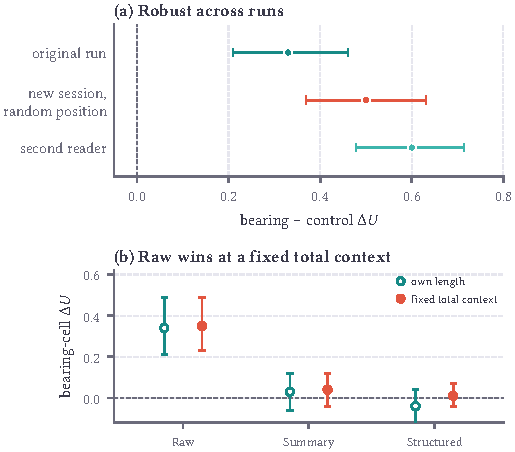
\includegraphics[width=\columnwidth]{fig_robust}
\caption{The bearing--control contrast remains positive across tested
conditions (LongMemEval-V2). \textbf{(a)}~Bearing minus
control, paired within memory, in the original run, in a new session with the
memory's position redrawn per replicate, and under a second reader (95\%
intervals over memories). \textbf{(b)}~Bearing-cell $\Delta U$ of each
representation at its own length ($n=\lcBearCells$) and with every arm padded to
the Raw arm's token count ($n=\soFN$, excluding cells exposed to a cache-key
defect); task-clustered intervals. Pre-registered: the original run and the
second reader in (a); exploratory: the new session in (a) and panel (b).}
\label{fig:robust}
\Description{Two panels. Top: three interval estimates of the bearing-minus-control effect, for the original run, a new session with random position, and a second reader, all well above zero. Bottom: Raw near 0.35 and Summary and Structured near zero, both at their own length and at a fixed total context.}
\end{figure}

\begin{table}[t]
\centering\small
\caption{Screened run on LongMemEval-V2: the same 60 memories paired with
three strata of tasks. Both-arms-fail is the fraction of cells in which the
reader fails with \emph{and} without the memory; such cells cannot show a
memory effect. The criterion for a material reduction (\textsc{bearing}'s
Wilson upper bound below the comparator's point estimate) was fixed in code
before these numbers existed.}
\label{tab:screened}
\begin{tabular}{@{}lrcr@{}}
\toprule
stratum & both-arms-fail & Wilson 95\% & mean $\Delta U$ \\
\midrule
\textsc{bearing}      & \textbf{0.53} & [0.44, \textbf{0.61}] & \textbf{\rd{\stratBearV}} \\
matched control       & 0.79 & [0.71, 0.85] & \rd{\stratCtrlV} \\
\textsc{random}       & 0.70 & [0.67, 0.73] & \rd{\stratRandV} \\
\bottomrule
\end{tabular}
\end{table}
The screened design reduces these structural zeros: cells that fail in both
arms fall to 0.53 for \textsc{bearing}, against 0.79 for the matched control and
0.70 for \textsc{random} (Table~\ref{tab:screened}). The memory helped in
$\spBearPos$ of $\spBearN$ \textsc{bearing} cells ($\spBearRate\%$), against
$\spCtrlRate\%$ for the control and $\spRandRate\%$ for \textsc{random}, and
$\spZeroPct\%$ of all $\spCells$ cells are exact zeros.

\textbf{The headline contrast.} For each memory, we compare its mean paired
reward gain on answer-bearing task pairs with its mean gain on matched-control
task pairs. Averaged over the $\lfHeadMems$ memories, this contrast is $\lfHeadD$ $[\lfHeadLo, \lfHeadHi]$
(episode-clustered $[\lfHeadEpLo, \lfHeadEpHi]$; two-way over memories and
tasks $[\rd{\lfTwoWayLo}, \rd{\lfTwoWayHi}]$; Figure~\ref{fig:robust}a).
It is similar for single-task ($\rvHeadSingle$) and multi-task
($\rvHeadMulti$) memories, and $\rvHeadW$ $[\rvHeadWLo, \rvHeadWHi]$ reweighted
to all $\rvPopAll$ bearing memories.
It differs from the bearing stratum's own mean $\Delta U$ in
Table~\ref{tab:screened}, which is not paired within memory.
Because the screen selects pairs whose memory contains the answer, this result
first validates the instrument: the protocol detects the effect it should.

\textbf{The contrast holds across session, position and reader.} Re-running all
$\soXoneCells$ bearing and control cells in a new session, three replicates each
with the memory's position redrawn ($\soXoneCalls$ calls, none from cache),
gives $\soXoneD$ $[\soXoneLo, \soXoneHi]$; under a second reader it is
$\rd{\rgBmcRawGem}$ (Section~\ref{sec:readertransfer}). The contrast keeps its
direction in every tested condition, while its magnitude moves with session and
reader, as Section~\ref{sec:limitations} anticipates.

Two checks address alternative explanations. First, the screen did not
select easier tasks. Because reward is binary, Table~\ref{tab:screened} and the
cell counts fix each stratum's accuracy without the memory: $\raAccZeroBear\%$
for \textsc{bearing}, $\raAccZeroCtrl\%$ for the control and
$\raAccZeroRand\%$ for \textsc{random}. Bearing tasks are the hardest without
the memory and the easiest with it ($\raAccOneBear\%$). The
$\raHurtOppBear$ bearing cells answered correctly without the memory
($\raBothCorrectBear$ of them also with it) show that the answer is sometimes
recoverable from the filler or from the reader's priors. Second, the reader can retrieve planted content: a unique code planted inside the target
memory, in the full $\sim$27k-token context, is recovered in 22 of 22 cells
and in 0 of 17 when nothing is planted (\supp{sec:needle}). This makes a simple
inability to access the long context less likely as the cause of low accuracy
on unscreened pairs.

\textbf{With the answer in context, the reader still fails on
$\raFailWithBearPct\%$ of bearing cells.} The planted-code test makes a simple
inability to access the context less likely, while failures to localize or use
natural evidence remain possible. These failures occur across question families (\supp{sec:lengthcontrol}).
Neither scorer leniency nor output truncation explains this pattern: every bearing pair matches the gold answer exactly ($\rvMatchExact$) or after
normalization ($\rvMatchNorm$), none by loose phrase containment, and exact
matches fail more often ($\rvFailExactPct\%$ against $\rvFailNormPct\%$).
Truncated outputs are re-run, not scored ($\rvRetried$ of $\rvScrRows$ rows).

\subsection{Retrievers find answer-bearing memories, but miss most}
\label{sec:similarity}
\begin{figure}[t]
\centering
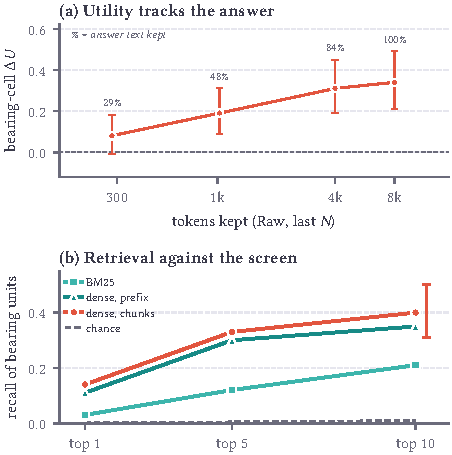
\includegraphics[width=\columnwidth]{fig_mech}
\caption{What carries utility (LongMemEval-V2). \textbf{(a)}~Bearing-cell
$\Delta U$ as Raw is cut to its last $N$ tokens ($\lcBearCells$ cells,
task-clustered intervals); labels give the share of cells whose text still
contains the answer. \textbf{(b)}~Share of a task's bearing units that a
retriever ranks in its top 1, 5 and 10 of the domain pool ($\soScrDisc$ tasks;
task-clustered interval shown at top 10); the dashed line is chance. Both panels are
exploratory; the matched-length contrast in (a) was pre-registered.}
\label{fig:mech}
\Description{Two panels. Top: bearing-cell utility rising with the number of Raw tokens kept, with the share of cells keeping the answer rising from 29 to 100 percent. Bottom: recall at ten for BM25, prefix and chunked dense retrieval, from 0.21 to 0.40, far above a near-zero chance line.}
\end{figure}
The screen defines which units of a domain pool are answer-bearing for each
of the $\soScrDisc$ tasks, so these screen-defined labels can score retrievers
that never see the answer (Figure~\ref{fig:mech}b). Recall@10 measures recovery
of these units, not of every helpful memory or the accuracy of a complete
retrieval system. Ranking the whole pool of $\lfPoolWeb$ or $\lfPoolEnt$ units by
the question, dense retrieval with SFR-Embedding-Mistral ranks, on average,
$\soRChkTen$ $[\soRChkTenLo, \soRChkTenHi]$ of a task's bearing units in its top
ten (recall@10) when units are split into 512-token chunks, and $\soRPreTen$ when
only a 2{,}000-token prefix is embedded, against about $\soChanceTenP$ by chance.
The lexical ranker BM25 reaches $\soRBmTen$, with an area under the ROC curve
(AUROC) of $\soRBmAuc$. Chunked retrieval places the first
bearing unit at a mean reciprocal rank of $\soRChkMrr$, and chunking improves recall only modestly over prefix embedding in this
comparison. Retrieval thus locates bearing
memories far above chance yet misses most of them in its top ten, which is why
a deployable locator remains open. Similarity is a weaker guide to how
\emph{much} a memory helps: across executed cells, cosine similarity correlates
with $\Delta U$ at only $\rho=\rd{\simRhoAll}$ (\supp{sec:simdetail}).

\subsection{Evaluated compressed representations gain less than Raw}
\label{sec:repr}
We repeat the measurement on the same experiences and tasks, changing only how
each experience is written down. On the $\frCells$ cells evaluated under all
three representations, the paired \textsc{bearing}$-$control effect is
$\rd{\frRawDU}$ for Raw (95\% CI $[\rd{\frRawLo}, \rd{\frRawHi}]$).
For Summary it is $\rd{\frSumDU}$ ($[\rd{\frSumLo}, \rd{\frSumHi}]$), and
for Structured it is $\rd{\frStrDU}$ ($[\rd{\frStrLo}, \rd{\frStrHi}]$)
(Figure~\ref*{S-fig:overview}d in the supplement). Only Raw excludes zero. Per cell, Summary exposes
a mean $\frSumTokExp$ tokens, Structured $\frStrTokExp$ and Raw $\frRawTokExp$.
This Raw contrast comes from a different run and memory set than the screened
one (Table~\ref{tab:coverage}); the intervals overlap.

\textbf{The pre-registered length control.} A content-blind \emph{extractive
truncation} keeps the final $N$ tokens of the same segment, with $N$ set per cell to that
cell's Summary length. On the $\lcBearCells$ bearing cells (task-clustered over
$\lcBearTasks$ tasks), the extractive and Summary arms differ by $\rd{\lcPrimary}$
$[\rd{\lcPrimaryLo}, \rd{\lcPrimaryHi}]$, which does not establish equivalence,
and Raw beats the matched extractive arm by $\rd{\lcBudget}$
$[\rd{\lcBudgetLo}, \rd{\lcBudgetHi}]$. Keeping the first $N$ tokens instead of the last,
the contrast registered as decisive, retains the bearing content in 0.7\% of
cells against 28.9\%; last-$N$ exceeds first-$N$ by $\rd{\lcEnds}$
$[\rd{\lcEndsLo}, \rd{\lcEndsHi}]$.



\textbf{A budget sweep.} The same run also
truncated Raw to its last 4,096 and 1,024 tokens (Figure~\ref{fig:mech}a).
Bearing-pair gains fall with the budget, $\lcRawM$, $\lcFourM$, $\lcOneM$ and $\lcMatchM$
from full length down to matched length, and the share of cells whose text
still contains the bearing content falls with it: $\lcRawKept\%$,
$\lcFourKept\%$, $\lcOneKept\%$ and $\lcMatchKept\%$. Splitting every arm by
whether its text kept that content (Figure~\ref*{S-fig:lenctl}b), the arms look
alike: cells that kept it gain $\lcPoolKeptM$ $[\lcPoolKeptLo, \lcPoolKeptHi]$
pooled over the compressed arms, Summary included at $\lcSumKM$, and cells that
lost it gain $\lcPoolLostM$ $[\lcPoolLostLo, \lcPoolLostHi]$. The cells that
kept the content are not simply easier: on the very same cells, Raw gains
$\lcSelSumKept$ where Summary kept it and $\lcSelSumLost$ where Summary lost it.
Structured is the exception, at $\lcStrKM$ on $\lcStrKN$ cells, but those are
cells where even Raw gains only $\lcSelStrKept$. Within Raw, $\Delta U$ correlates weakly with memory length across bearing
cells ($r = \lcRawLenR$), which does not by itself establish the absence of a
length effect. Under the evaluated task-blind writing strategies, compressed
representations often omit answer-bearing text and show smaller reward gains
than Raw; because the sweep changes content and length together, it is
consistent with, rather than proof of, retention of answer-bearing content
driving the gains. These analyses are
exploratory (session caveats in \supp{sec:lengthcontrol}). The phrase matcher may miss paraphrased answers. However, Summary cells
classified as having lost the answer-bearing content help in only
$\lcLostHelpSum$ of $\lcLostNSum$. The result describes one task-blind writer
and prompt, whose structured schema targets procedural lessons; a writer told to
keep values and identifiers might keep more bearing content.

\textbf{Raw retains its advantage at a fixed total context.} In deployment the main
argument for compression is that a long raw memory displaces other context. We
re-ran the $\soXtwoCells$ representation cells with every arm of a cell given
the same token count: the compressed arms and the no-memory arm were padded with
further bearing-disjoint filler (median $\soXtwoPad$ tokens) up to the Raw arm's
total, the memory kept at its original position. On bearing cells Raw gains
$\soFRaw$ $[\soFRawLo, \soFRawHi]$, while Summary gains $\soFSum$ and Structured
$\soFStr$; against Raw on the same cells they lose $\soFSumR$
$[\soFSumRLo, \soFSumRHi]$ and $\soFStrR$ $[\soFStrRLo, \soFStrRHi]$. Including
cells exposed to a cache-key defect changes no conclusion (\supp{sec:sophia};
Figure~\ref{fig:robust}b). Costs depend on the accounting: amortizing the
writer's one-time cost over this design's $\frReuse$ evaluated uses per memory
removes compression's token advantage, and Summary overtakes Raw on point
estimates only above about $\raReuseStar$ uses per write, with a utility
interval spanning zero throughout (\supp{sec:reuse}).

\subsection{The contrast keeps its direction under a second reader}
\label{sec:readertransfer}
One concern is that the Raw effect is specific to one reader. We re-executed
the $\lfSmCellsAll$ Raw bearing and control cells with a second, unrelated reader
(gemma-4-31B-it) on the same memory text. The memory file, prompt, filler,
every rendered request and each target position were hash-asserted against
the first run, and the text re-verified byte-identical on $\rgRows$ rows.
Because this endpoint is not deterministic across sessions
(Section~\ref{sec:limitations}), we ran both readers in one session and quote
that measurement.

The aggregate contrast keeps its direction and is larger: over $\rgSmCells$ matched cells on
$\rgSmTasks$ tasks, the second reader's mean $\Delta U$ is higher by
$\rd{\rgSmDiff}$ $[\rd{\rgSmLo}, \rd{\rgSmHi}]$, and the within-memory
\textsc{bearing}$-$control contrast is $\rd{\rgBmcRawGem}$
(Figure~\ref{fig:robust}a). Part of the gain comes
from a weaker no-memory arm under the second reader ($\rd{\rgWithoutDelta}$)
rather than from a better memory.

\textbf{The aggregate contrast retains its direction across the two readers,
while per-pair labels show partial agreement.} Over the
$\rgSmCells$ cells, the two readers' three-way labels (helped, unchanged,
hurt) agree at Cohen's $\kappa = \raReaderKappa$. Of the $\raReaderMoving$
cells that move under either reader, both mark $\smAgree$ as helped
(Figure~\ref*{S-fig:overview}f). Too few cells are harmed ($\raHurtOss$ and
$\raHurtGem$) to tell whether harm labels reproduce. Whether a reader favors memories its own model
wrote is tested by a pre-registered writer\,$\times$\,reader factorial crossing
both models as writers and readers. On Summary and Structured, whose utility
is already near zero, the factorial excludes writer and same-family effects above $0.038$
(\supp{sec:readerfull}).

\subsection{What the instrument did not find}
\label{sec:r0}
\begin{figure}[t]
\centering
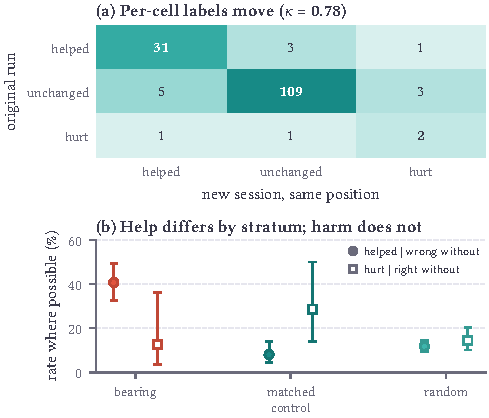
\includegraphics[width=\columnwidth]{fig_cells}
\caption{What single cells can and cannot show (exploratory).
\textbf{(a)}~Per-cell labels (helped, unchanged, hurt) in the original run
against a new session at the same memory position ($\soStabSameN$ replicate
cells; diagonal agrees). At a new position $\kappa$ falls to $\soStabDiffK$, and
between two readers it is $\raReaderKappa$.
\textbf{(b)}~Help among cells the reader got wrong without the memory (filled)
and harm among cells it got right (hollow), by stratum, Wilson 95\% intervals:
help differs sharply, harm does not detectably.}
\label{fig:cells}
\Description{Two panels. Top: Cohen's kappa of 0.78, 0.65 and 0.58 for a new session at the same position, a new session at a new position, and a second reader, with 91, 87 and 82 percent raw agreement. Bottom: help rates of about 41 percent for bearing against 8 and 12 percent for control and random, while harm rates overlap across strata.}
\end{figure}
The study was designed to measure sign reversal: one memory helping one task
and harming another. Two naive comparisons mislead. Flip rates depend on cells
per memory ($\raCellsPerMemBear$ for \textsc{bearing}, $\raCellsPerMemRand$ for
\textsc{random}): at matched counts and no-memory outcomes, \textsc{random} also
shows no flip in $\lfCondFlipPZero\%$ of resamples. And harm shares depend on
baseline accuracy, since a memory can only hurt where the reader was right
without it. Conditioning on that opportunity (Figure~\ref{fig:cells}b;
\supp{sec:negative}), answer-bearing
pairs hurt in $\raHurtRateBear\%$ $[\raHurtLoBear, \raHurtHiBear]$ of the
$\raHurtOppBear$ baseline-correct pairs where they could, random-task pairs in
$\raHurtRateRand\%$ $[\raHurtLoRand, \raHurtHiRand]$: \emph{we detect no excess
harm}, but with 16 pairs the design could detect only a bearing harm rate of
$\rvHarmMdePct\%$ or more, so this does not establish the absence of harm. Matched-control pairs hurt in
$\raHurtRateCtrl\%$ $[\raHurtLoCtrl, \raHurtHiCtrl]$, an interval that overlaps
random's. The strata
differ in help: $\raHelpRateBear\%$ $[\raHelpLoBear, \raHelpHiBear]$ of the
cells where the reader was wrong, against $\raHelpRateRand\%$ for
\textsc{random}. The planned variance decomposition is not identifiable in the main run
(exploratory estimate in \supp{sec:sophia}).
